
\subsubsection{18.10.14}

\begin{enumerate}
	\item Time of beginning and ending of meeting:
	16:30 - 21:40
	\item Purposes of meeting:
	\begin{enumerate}
	  \item To create the finished version of gripper for balls.
	  
	  \item To change the programme of control of gripper to more comfortable.
	  
    \end{enumerate}
    
	\item Work that has been done:
	\begin{enumerate}
      
      \item Screeds were located at the axle in 4 rows through every 90 degrees and fixed by the hot-melt adhesive.
      
      \begin{figure}[H]
      	\begin{minipage}[h]{0.47\linewidth}
      		\center{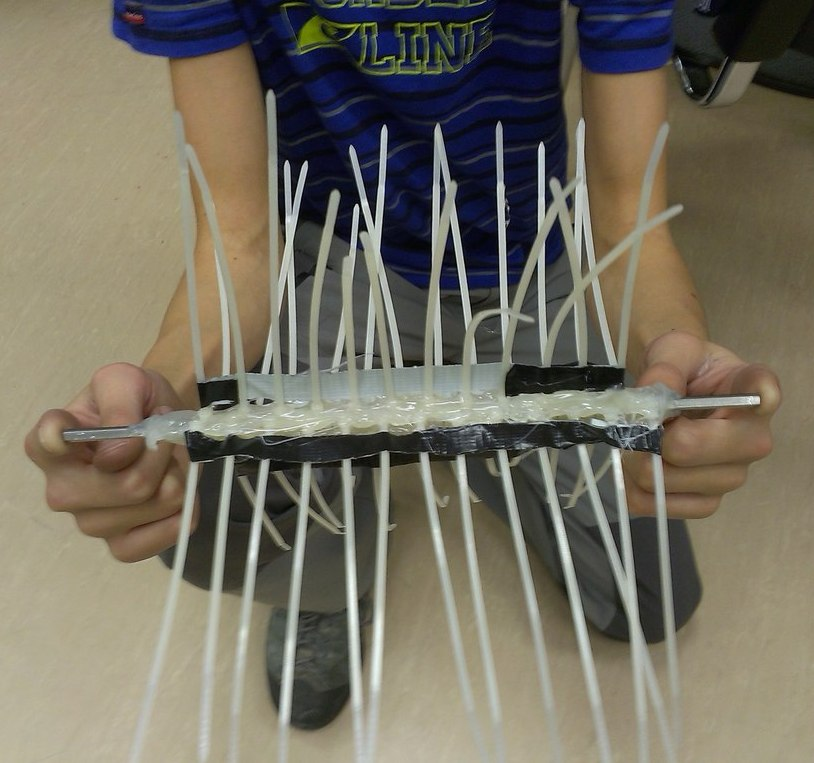
\includegraphics[scale=0.3]{days/18.10.14/images/01}}
      		\caption{Brush of gripper}
      	\end{minipage}
      	\hfill
      	\begin{minipage}[h]{0.47\linewidth}
      		\center{
\includegraphics[scale=0.3]{days/18.10.14/images/02}}
      		\caption{The finished version of gripper for balls}
      	\end{minipage}
      \end{figure}
      
      \item Programme of control of gripper was changed. Now servo changes state (stop or running) by pressing the button. It allows to operator don't distracted to maintaining of gripper at working condition.   
      
      \item Gripper was tested on two balls from NXT set diametr 5cm. Robot can to capture balls at the open space and near the walls. There was one problem: brush locates only at the center of robot and for capture of ball it need to aim to it. We planned to install on each side of the gripper beams located like a funnel (hereinafter they will be called as slopes) for solving this problem. It allows to balls to roll to gripper.
      
      \item It was turned out that when servo is stopping it try to keep angle,so it rattles. This needs to be corrected.
      
      \item It was turned out that robot stop to shake when it turns around. It happened because a large part of it's mass was concentrated in the back part of robot. So the front wheels slipped freely.
      
      \item In addition the start tasks it was made mechanism of overturning bucket.
      
      \begin{figure}[H]
      	\begin{minipage}[h]{1\linewidth}
      		\center{
\includegraphics[scale=0.2]{days/18.10.14/images/03}}
      		\caption{Mechanism of overturning bucket}
      	\end{minipage}
      \end{figure}
      
    \end{enumerate}
    
	\item Results: 
	\begin{enumerate}
	  \item The gripper was finished.
	  
      \item It was created more comfortable programme of control the gripper.
      
    \end{enumerate}
    
	\item Tasks for the next meetings:
	\begin{enumerate}
	  \item To correct the problem with servo.
	  
	  \item To install the slopes.

    \end{enumerate}     
\end{enumerate}
\fillpage
